%ChapterIV.tex
\section{模拟通信系统}\label{chapter:IV}
\HyperBack{chapter:IV}
\subsection{引言}
    模拟信号的特征是\emph{时间连续}、\emph{幅度连续},而且在本章中考虑的模拟信号一般没有直流分量,
    从信息传递的角度确定的直流信号不传递任何信息。

    为了想让将原始电信号变换成适合频带信道传输的信号,必须经过\emph{调制}。
    其方式是按调制信号的变化规律去改变载波的某些参数。
    一般使用\emph{正弦波}或者\emph{脉冲}作为载波进行调制。
    有三点作用:
    \begin{enumerate}[itemsep=0pt,parsep=0em,label=\color{bupt}\arabic*、,labelsep=0pt,leftmargin=4em]
        \item 匹配信道带同特性。
        \item 可以实现如频分复用等技术,提高效率。
        \item 采用不同调制方式可以兼顾通信的\emph{有效性}与\emph{可靠性}。
    \end{enumerate}
    
    \noindent 对于本章主要研究的正弦波模拟调制:
    即已调信号为$s_m(t)=A(t)\cos[2\pi f_ct+\varphi(t)]$

    \noindent 主要研究三种调制方法
    \paragraph{幅度调制:}$A(t)$随$m(t)$成比例变化。
    \paragraph{相位调制:}$\varphi(t)$随$m(t)$成比例变化。
    \vspace{-1ex}
    \paragraph{频率调制:}$\dfrac{\dif \varphi(t)}{\dif t}$随$m(t)$成比例变化。
    \vspace{3ex}

    其中第一种方法是线性调制,后两种统称角度调制,均为非线性调制。
    关于每种调制方法,从以下几方面中研究:
    \begin{enumerate}[itemsep=0pt,parsep=0em,label=\color{bupt}\arabic*、,labelsep=0pt,leftmargin=4em]
        \item 时域表达式。
        \item 频域表达式(频域特点)。
        \item 发射机模型。
        \item 接收机模型。
        \item 抗噪声性能分析 (解调输出信噪比)。
    \end{enumerate}

\subsection{幅度调制}
    AM,Amplitude Modulation

    幅度调制是正弦型载波的幅度随调制信号作\emph{线性}变化的过程,
    已调信号的频谱是调制信号的频谱的线性搬移,故为线性调制。

    幅度调制的一般模型是将信号$m(t)$和载波$\cos(2\pi f_ct)$相乘后通过单位冲激响应为$h(t)$的滤波器。
    依据$m(t)$和$h(t)$的不同可以分为以下四种:\footnote{以下的列表是嵌入超链接的局部目录,可以转跳到对应的小节。}
    \begin{enumerate}[itemsep=0pt,parsep=0em,label=\color{bupt}\arabic*、,labelsep=0pt,leftmargin=4em]
        \item \hyperref[subsubsec:DSB-SCAM]{双边带抑制载波调幅}
        \item \hyperref[subsubsec:AM]{标准调幅}
        \item \hyperref[subsubsec:SSB]{单边带调幅}
        \item \hyperref[subsubsec:VSB]{残留带调幅}
    \end{enumerate}

    \subsubsection{双边带抑制载波调幅}\label{subsubsec:DSB-SCAM}
    DSB-SC AM,Double Sideband-Suppressed Carrier Amplitude Modulation
    
    \paragraph{双边带抑制载波调制信号的产生}\mbox{}

    双边带抑制载波调幅信号$s(t)$是利用均值为零\footnote{或者说直流分量为零,即频谱在$f=0$处没有冲激函数,但可以是不为零的实数
    这也是抑制载波Suppressed Carrier的来源。}的的模拟基带信号$m(t)$与正弦载波$c(t)$相乘得到的。

    \begin{figure}[H]
        \centering
        \subcaptionbox*{(a)基带信号}[200pt][c]{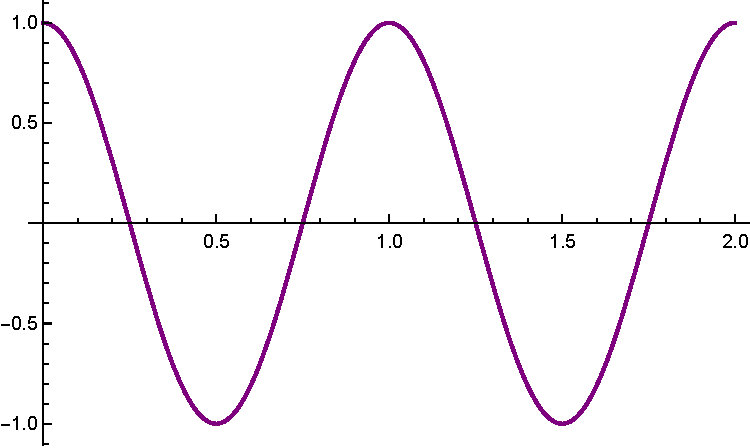
\includegraphics[scale=0.5]{body/image/book422a.pdf}}
        \subcaptionbox*{(b)已调信号}[200pt][c]{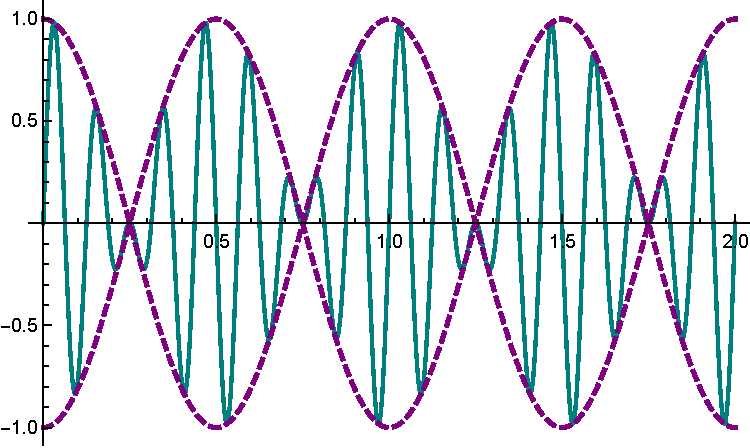
\includegraphics[scale=0.5]{body/image/book422b.pdf}}
        \caption{基带信号和已调信号波形}
    \end{figure}

    注意到有些地方载波和调制信号同时改变极性,称此点为\emph{反相点},其出现不改变性能。
    但是已调信号的幅度为上图中的紫色虚线,即$\abs{m(t)}$,相较于原信号,损失了原信号的\emph{极性},
    故不能从包络中还原原信号。
    
    \paragraph{频谱/功率谱特性}\mbox{}

    载波$s(t)=A\cos(2\pi f_ct)$的频谱为$S(f)=\dfrac{A}{2}[\delta(f-f_c)+\delta(f+f_c)]$,
    调制信号与之乘相当于把频谱向两侧平移。
    即对于带宽$W$的信号$m(t)\leftrightarrow M(t)$有
    \begin{equation}
        s_m(t)=m(t)s(t)\leftrightarrow\frac{A}{2}[M(f-f_c)+M(f+f_c)]
    \end{equation}
    如下图所示
    \begin{figure}[H]
        \centering
        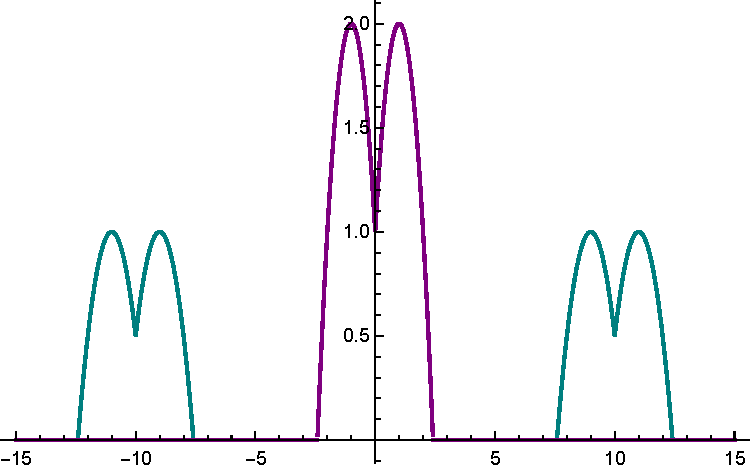
\includegraphics[width=400pt,height=70pt]{body/image/book423.pdf}
        \caption{频谱搬移示意图}
    \end{figure}

    可见其带宽被展宽了二倍。但如果调制信号$m(t)$是实函数,
    称$\abs{f}\in[f_c-W,f_c]$的部分为\emph{下边带};称$\abs{f}\in[f_c,f_c+W]$的部分为\emph{上边带}。
    调制信号的上下边带是\emph{关于$f_c$的两侧是共轭对称的},
    从信息量上看,相当于信息的冗余,降低了有效性。
    如果仅留一个边带则是后文\hyperref[subsubsec:SSB]{单边带调幅}的内容

    对于功率谱,如果$M(t)$是零均值平稳过程。
    有$R_M(\tau)\leftrightarrow P_M(f)$。
    对于已调信号
    \begin{equation}
        S(t)=A_cM(t)\cos(2\pi f_c t)
    \end{equation}

    均值
    \begin{equation}
        m_S(t)\mathscr{E}[S(t)]=A_c\mathscr{E}[M(t)]\cos(2\pi f_c t)=0
    \end{equation}

    自相关函数
    \begin{equation*}
        \begin{split}
            R_S(t,\tau)&=\mathscr{E}[S(t+\tau)S^*(t)]\\
                     &=A_c^2\mathscr{E}[M(t+\tau)M^*(t)]\mathscr{E}[\cos(2\pi f_c t)\cos(2\pi f_c t+2\pi f_c \tau)]\\
                     &=\frac{A_c^2}{2}R_M(\tau)[\cos(2\pi f_c \tau)+\cos(4\pi f_c t+2\pi f_c \tau)]
        \end{split}
    \end{equation*}

    可见已调信号不是平稳过程,是周期平稳过程。由\eqaref{eq:avgRXtau}得平均自相关函数
    \begin{equation}
        \begin{split}
            \overline{R_S}(t,\tau)&=\lim_{T\to\infty}\left[\frac{1}{T}\int_{-\frac{T}{2}}^{\frac{T}{2}}R_S(t,\tau)\dif t\right]\\
                                  &=\frac{A_c^2}{2}\cos(2\pi f_c \tau)\lim_{T\to\infty}\left[\frac{1}{T}\int_{-\frac{T}{2}}^{\frac{T}{2}}R_M(\tau)\dif t\right]\\
                                  &\phantom{=}+\frac{A_c^2}{2}\lim_{T\to\infty}\left[\frac{1}{T}\int_{-\frac{T}{2}}^{\frac{T}{2}}R_M(\tau)\cos(4\pi f_c t+2\pi f_c \tau)\dif t\right]
        \end{split}
    \end{equation}
    考虑其平稳性,$\overline{R_S}(t,\tau)=\dfrac{A_c^2}{2}R_M(\tau)\cos(2\pi f_c \tau)$,
    由\hyperref[thm:Wiener_Khinchin]{维纳--辛钦定理}得
    \begin{equation}\label{eq:DSB-SCAM-P}
            \overline{P_S}(f)=\mathscr{F}[\overline{R_S}(\tau)]=\frac{A_c^2}{4}[P_M(f-f_c)+P_M(f+f_c)]                        
    \end{equation}
    
    对于非平稳的$M(t)$,如果$M(t)$变化缓慢,即$W\ll f_c$,仍近似有\footnote{可以从这个角度理解:如果变化缓慢,说明没有高频分量,与余弦函数相乘之后,其频谱都被平移到高频,时域上的面积,即频域上原点的值,为零。}
    \begin{equation}
        \lim_{T\to\infty}\left[\frac{1}{T}\int_{-\frac{T}{2}}^{\frac{T}{2}}R(t,\tau)\cos(4\pi f_c t+2\pi f_c \tau)\dif t\right]=0
    \end{equation}
    上述结论仍成立。

    \paragraph{相干解调(Coherent Demodulation)}\mbox{}

    在这一部分中先不考虑噪声的问题,假设收到的信号$r(t)=A_cm(t)\cos(2\pi f_ct +\varphi_c)$,使用$\cos(2\pi f_c +\varphi)$与之相乘并通过低通滤波器,得到
    \begin{equation}
        \begin{split}
            y_o(t)&=[A_cm(t)cos(2\pi f_ct +\varphi_c)\cos(2\pi f_ct +\varphi)]_{LPF}\\%FIXME:杨欣洁小姐姐第一次的问题反馈!
                  &=\frac{A_c}{2}m(t)cos(\varphi-\varphi_c)
        \end{split}
    \end{equation}

    更进一步的,如果把$r(t)$写成同相分量和正交分量的形式,即$r(t)=r_c(t)cos(2\pi f_ct)$ $-r_s(t)\sin(2\pi f_ct)$,相干解调后的结果实际上是$r_c(t)$,即同相分量。

    为了尽可能使接收到的信号尽可能地大,需要与接收到的信号的载波\emph{同频同相位},即相干\footnote{这个概念是从光学干涉那里借鉴过来的。}。
    可以使用\emph{导频法}。

    在调制信号中增加直流分量,在频域上表现为一个离散的冲激函数。
    发射信号变为
    \begin{equation}
        s(t)=A_cm(t)\cos(2\pi f_ct)+A_p\cos(2\pi f_ct)
    \end{equation}
    在接收端用\emph{窄带滤波器}提取出来作为相干载波。
    但要注意\emph{导频的功率要求比调制信号的功率小}(这是与有大离散载波的调幅信号的区别所在),

    \subsubsection[标准调幅]{标准调幅/包络调制}\label{subsubsec:AM}
    在\hyperref[subsubsec:DSB-SCAM]{双边带抑制载波调幅}中,接收机需要解调电路,如提取导波,或者使用平方环法、COSTAS环法等不需要导频的非线性方法提取载波,
    但仍然会提高接收机成本,故标准调幅AM使用大功率离散载波,可以使用包络检波器进行解调,接收机成本低。大功率离散载波造成的成本问题由广播电台解决。
    
    \paragraph{标准调幅信号的产生}\mbox{}

    使用大离散载波,在调制信号上叠加强度为$A_0$的直流分量,把已调信号平全部移到横轴上方,保证已调信号的包络在几乎任意时刻不为零\footnote{以概率1不等于0},不会出现因为极性突变而不能由已调信号还原调制信号包络的问题。

    \begin{figure}[H]
        \centering
        \subcaptionbox*{(a)基带信号}[200pt][c]{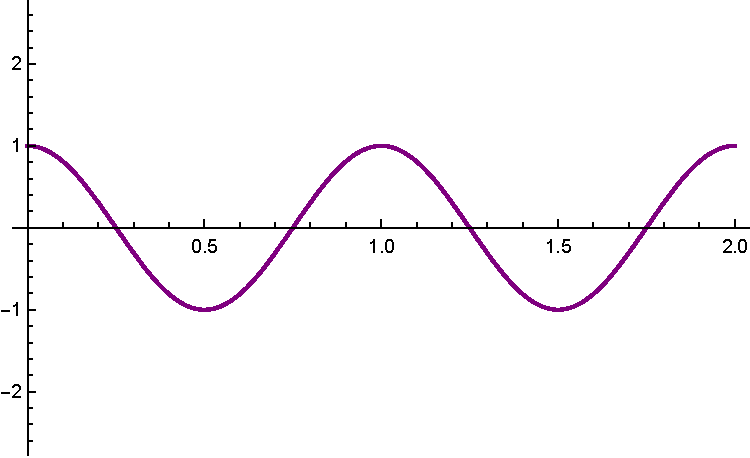
\includegraphics[scale=0.5]{body/image/book426AMmt.pdf}}
        \subcaptionbox*{(b)已调信号}[200pt][c]{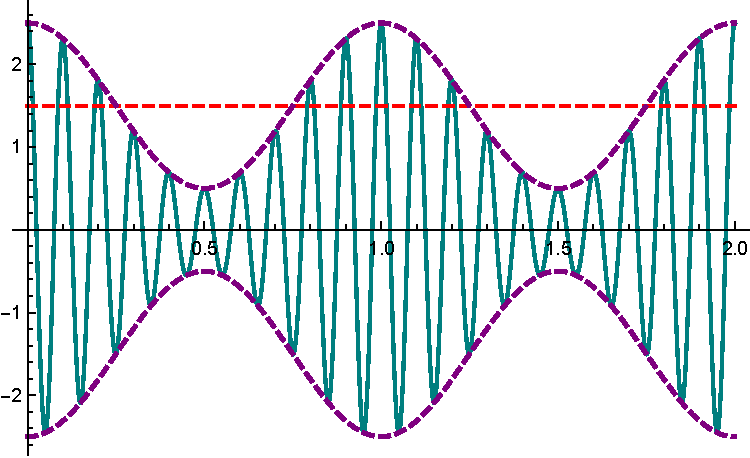
\includegraphics[scale=0.5]{body/image/book426AMst.pdf}}
        \caption{基带信号和已调信号波形}
    \end{figure}

    上图中左侧为调制信号,右图中松绿色线为已调信号,紫色虚线为其包络,红色则是离散载波的幅度$A_0$。
    
    输出信号$s(t)=[A_0+A'm(t)]\cos(2\pi f_ct)$,不难知需要满足$A_0\geq A'\abs{m(t)}$。记
    \begin{equation}
        a=\frac{A'\text{max}\abs{m(t)}}{A_0}\leq 1
    \end{equation}
    为\emph{调制指数}或\emph{调幅系数},那么输出信号可以写作
    \begin{equation}
        s(t)=A_0[1+am_n(t)]\cos(2\pi f_ct)
    \end{equation}
    其中$m_n(t)=\dfrac{m(t)}{\text{max}\abs{m(t)}}$,是$m(t)$的归一化表示。

    \paragraph{频谱/功率谱特性}\mbox{}

    对于确定信号$m_n(t)\leftrightarrow M_n(f)$
    \begin{equation}
        S(f)=\frac{A_0}{2}[\delta(f-f_c)+aM_n(f-f_c)]+\frac{A_0}{2}[\delta(f+f_c)+aM_n(f+f_c)]
    \end{equation}
    
    推广到零均值平稳随机过程$M(t)$,$S(t)=[A_0+A'M(t)]\cos(2\pi f_ct)$
    均值
    \begin{equation}
        \mathscr{E}[S(t)]=A_0\cos(2\pi f_ct)
    \end{equation}
    平均自相关函数
    \begin{equation}
        \overline{R_S}(\tau)=\frac{1}{2}[A_0^2+A'^2R_M(\tau)]\cos(2\pi f_c\tau)
    \end{equation}
    已调信号同样为周期平稳过程,不难知
    \begin{equation}
        P_S=\frac{A_0^2}{2}+\frac{A'^2}{2}P_M=\frac{A_0^2}{2}+\frac{\overline{\abs{A'm(t)}^2}}{2}
    \end{equation}

    因为$A_0\geq A'\abs{m(t)}$,至少有一半发射功率是分配给离散的载频分量,功率效率低!

    可以定义\emph{携带信息的已调信号功率与已调信号总功率之比}
    \begin{equation}
        \eta=\frac{\dfrac{A'^2P_m}{2}}{\dfrac{A_0^2}{2}+\dfrac{A'^2P_m}{2}}=\frac{a^2P_{m_n}}{1+a^2P_{m_n}}
    \end{equation}
    其中$P_{m_n}$是归一化信号$m_n(t)$的功率

    \paragraph{信号解调}\mbox{}

    因为信号包络没有极性突变,故可以使用价位更加低廉的包络检测器,
    其原理总体上为:先用整流电路将赋值小于零的部分翻转上来(或归零),
    再通过低通滤波,得到$A_0+A'm(t)$,滤掉直流分量即得到输出$y_0(t)=A'm(t)$。
    这种解调方法属于非相干解调。

    \subsubsection{单边带调幅}\label{subsubsec:SSB}
    双边带调幅(DSB、AM)的频谱有两个对称的边带,其带宽是基带信号的二倍。
    因为两个边带是共轭对称的,故可以去掉一个边带进行传输。

    \paragraph{信号的产生}\mbox{}
    
    如上边带调制,就将$s(t)=2A_cm(t)\cos(2\pi f_ct)$通过一个理想高通滤波器,其下截止频率为$f_c$。
    $m(t)\cos(2\pi f_ct)$的复包络为
    \begin{equation}
        s_L(t)=A_c[m(t)+j\hat{m}(t)]
    \end{equation}
    滤波器的等效基带传递函数为
    \begin{equation}
        H(f)=\left\{
        \begin{aligned}
            1,\hspace{1em}f\geq 0\\
            0,\hspace{1em}f< 0
        \end{aligned}   
        \right.
        =\frac{1+\text{sign}(f)}{2}
    \end{equation}
    由\hyperref[subsec:bandsystem]{等效带通系统}的知识可以知道,
    上下边带信号可以表示为
    \begin{align}
        s_{\text{上}}(t)&=A_cm(t)\cos(2\pi f_ct)-A_c\hat{m}(t)\sin(2\pi f_ct)\\
        s_{\text{下}}(t)&=A_cm(t)\cos(2\pi f_ct)+A_c\hat{m}(t)\sin(2\pi f_ct)
    \end{align}
    
    \begin{figure}[H]
        \centering
        \subcaptionbox*{(a)基带信号}[200pt][c]{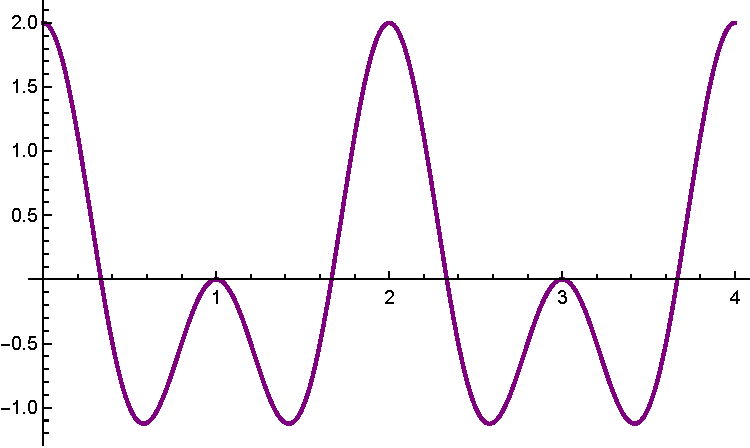
\includegraphics[scale=0.5]{body/image/chap4SSBa.pdf}}
        \subcaptionbox*{(b)DSB已调信号}[200pt][c]{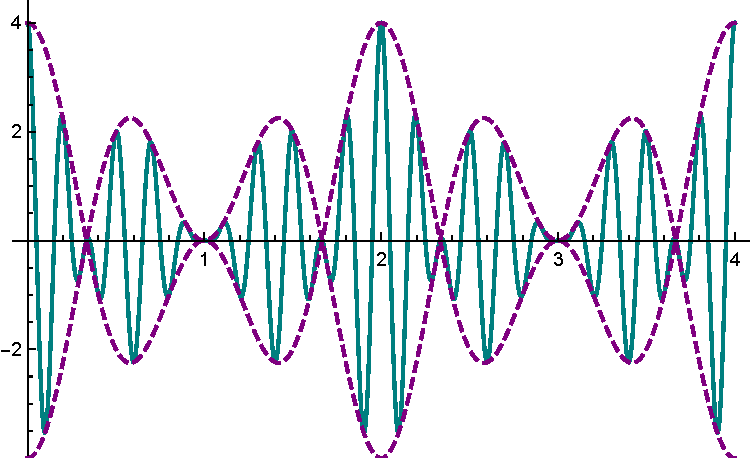
\includegraphics[scale=0.5]{body/image/chap4SSBb.pdf}}

        \subcaptionbox*{(c)上边带信号}[200pt][c]{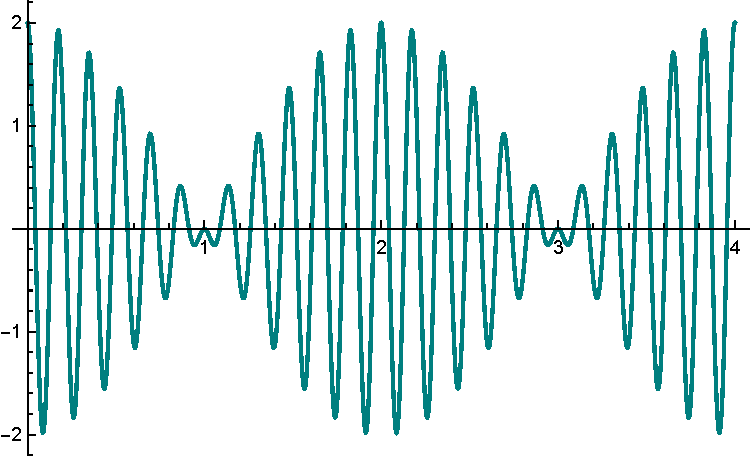
\includegraphics[scale=0.5]{body/image/chap4SSBc.pdf}}
        \subcaptionbox*{(d)下边带信号}[200pt][c]{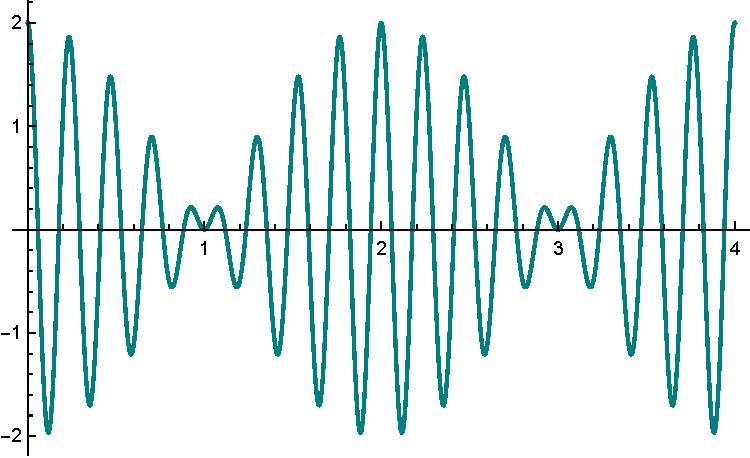
\includegraphics[scale=0.5]{body/image/chap4SSBd.pdf}}
        \caption{基带信号和已调信号波形}
    \end{figure}

    \paragraph{频谱/功率谱特征}\mbox{}

    对于基带随机平稳过程$M(t)$,其自相关函数和功率谱密度为$R_M(\tau)\leftrightarrow P_M(f)$。
    以上边带为例,已调信号$S(t)$的自相关函数为
    \begin{equation*}
        \begin{split}
            R_S(t,\tau) &=\mathscr{E}[S(t+\tau)S^*(t)]\\
                        &=\mathscr{E}\{[A_cM(t+\tau)\cos(2\pi f_ct+2\pi f_c\tau)-A_c\hat{M}(t+\tau)\sin(2\pi f_ct+2\pi f_c\tau)]\\
                        &\phantom{=\mathscr{E}}\cdot[A_cM(t)\cos(2\pi f_ct)-A_c\hat{M}(t)\sin(2\pi f_ct)]\}\\
                        &           =\frac{A_c^2}{2}\mathscr{E}[M(t+\tau)M(t)]            [\cos(4\pi f_ct+\tau)+\cos(2\pi f_c\tau)]\\
                        &\phantom{=}+\frac{A_c^2}{2}\mathscr{E}[\hat{M}(t+\tau)\hat{M}(t)][-\cos(4\pi f_ct+\tau)+\cos(2\pi f_c\tau)]\\
                        &\phantom{=}-\frac{A_c^2}{2}\mathscr{E}[\hat{M}(t+\tau)M(t)]      [\sin(4\pi f_ct+\tau)+\sin(2\pi f_c\tau)]\\
                        &\phantom{=}-\frac{A_c^2}{2}\mathscr{E}[M(t+\tau)\hat{M}(t)]      [\sin(4\pi f_ct+\tau)-\sin(2\pi f_c\tau)]
        \end{split}
    \end{equation*}
    由\hyperref[subsubsec:LITsystem]{平稳过程通过线性系统}的内容
    \begin{align}
        &R_{\hat{M}}(\tau)=\mathscr{E}[\hat{M}(t+\tau)\hat{M}(t)]=R_{M}(\tau)\\
        &R_{\hat{M}M}(\tau)=R_{M}(\tau)*h(\tau)=\hat{R_{M}}(\tau)\\
        &R_{M\hat{M}}(\tau)=R_{\hat{M}M}(-\tau)=\hat{R_{M}}(-\tau)=-\hat{R_{M}}(\tau)
    \end{align}
    不难得到
    \begin{equation}
        R_S(t,\tau)=  A_c^2[R_M(\tau)\cos(2\pi f_c\tau)-\hat{R_{M}}(\tau)\sin(2\pi f_c\tau)]
    \end{equation}
    做傅里叶变换,得到其频谱
    \begin{equation}
        \begin{split}
            P_S(f)  &=\frac{A_c^2}{2}P_M(f)*[\delta(f-f_c)+\delta(f+f_c)]\\
                    &\phantom{=}+\frac{A_c^2}{2}[P_M(f)\text{sign}(f)]*[\delta(f-f_c)-\delta(f+f_c)]\\
                    &=\frac{A_c^2}{2}P_M(f-f_c)[1+\text{sign}(f-f_c)]+\frac{A_c^2}{2}P_M(f+f_c)[1-\text{sign}(f+f_c)]\\
                    &=A_c^2P_M(f-f_c)u(f-f_c)+A_c^2P_M(f+f_c)u(-f-f_c)
        \end{split}
    \end{equation}

    \paragraph{相干解调}\mbox{}

    与同频同相的$\cos(2\pi f_ct)$相干解调的结果为
    \begin{equation}
        y_o(t)=\frac{A_c}{2}m(t)
    \end{equation}
    特别的,如解调信号与接收信号有$\varphi$的相位差,即$\cos(2\pi f_ct+\varphi)$,
    由和差化积不难知道,上下边带信号的解调结果分别是
    \begin{align}
        y_{\text{上}}(t)&=\frac{A_c}{2}[m(t)\cos\varphi+\hat{m}(t)\sin\varphi]\\
        y_{\text{下}}(t)&=\frac{A_c}{2}[m(t)\cos\varphi-\hat{m}(t)\sin\varphi]
    \end{align}
    可见,如果解调信号没有相干,会引入正交分量的干扰。

    \subsubsection{残留边带调幅}\label{subsubsec:VSB}

    语音信号的频谱范围为300Hz--4000Hz,实际工程中可以使用\hyperref[subsubsec:SSB]{单边带调幅}进行模拟语音通话,
    滤波器以0--300Hz的范围作为过渡带。
    但对于模拟电视等图像传输,低频信号成分重要且丰富,那么需要使用的高通滤波器就需要在载频$f_c$附近有十分陡峭的频率特性。
    这一点对于滤波器可能是设计困难甚至是难以实现的,所以不完全切除另一个边带,而是保留一部分。

    设调制信号$m(t)$其频谱为$M(f)$,与$A_c\cos(2\pi f_ct)$相乘后,通过传递函数为$H_{\text{VSB}}(f)$的滤波器,
    频谱变为
    \begin{equation}
        S_{\text{VSB}}(f)=\frac{A_c}{2}[M(f-f_c)+M(f+f_c)]H_{\text{VSB}}(f)
    \end{equation}
    与$\cos(2\pi f_ct)$相乘相干解调得到
    \begin{equation}
        \begin{split}
            Y(f)&=\frac{A_c}{2}[M(f-2f_c)+M(f)]H_{\text{VSB}}(f-f_c)\\
                &\phantom{=}+\frac{A_c}{2}[M(f)+M(f+2f_c)]H_{\text{VSB}}(f+f_c)\\
        \end{split}
    \end{equation}
    通过低通滤波器后滤掉$\pm 2f_c$附近的的高频成分得到
    \begin{equation}
        Y_o(f)=\frac{A_c}{2}M(f)[H_{\text{VSB}}(f-f_c)+H_{\text{VSB}}(f+f_c)]
    \end{equation}
    为了能还原出$m(t)$,应该有
    \begin{equation}
        H_{\text{VSB}}(f-f_c)+H_{\text{VSB}}(f+f_c)=\text{const},\hspace{1em}\abs{f}<B  
    \end{equation}

\subsection{线性调制系统的抗噪声性能}
    假设已调信号在信道中传输的时候叠加上一高斯白噪声,
    其单边功率谱密度为$\dfrac{N_0}{2}$。
    接收后通过一\emph{等效噪声带宽}为B的带通滤波器。
    高斯白噪声变为\hyperref[subsubsec:BAWGN]{窄带平稳高斯白噪}。
    即接收信号
    \begin{equation}
        r(t)=s(t)+[n_c(t)\cos(2\pi f_ct)-n_s(t)\sin(2\pi f_ct)]
    \end{equation}
    其中$n_c(t)$、$n_s(t)$是窄带噪声的同相分量和正交分量。二者带宽均为$\dfrac{B}{2}$,功率谱密度为$N_0$。

    \subsubsection{DSB-SC AM系统的抗噪声性能}
    设接收到的信号为
    \begin{equation}
        r(t)=A_cm(t)\cos(2\pi f_ct)+[n_c(t)\cos(2\pi f_ct)-n_s(t)\sin(2\pi f_ct)]
    \end{equation}
    由\eqaref{eq:DSB-SCAM-P},信号功率为$P_R=\dfrac{A_c^2}{2}P_m$,
    噪声带宽为2B,噪声功率为$P_{n_i}=2N_0B$
    输入信噪比为
    \begin{equation}
        \left(\frac{S}{N}\right)_{i\text{,DSB}}=\frac{A_c^2P_m}{4N_0B}
    \end{equation}

    若本地解调载波为$2\cos(2\pi f_ct+\varphi)$,
    解调信号
    \begin{equation}
        y_o(t)=A_cm(t)\cos\varphi+[n_c(t)\cos\varphi+n_s(t)\sin\varphi]
    \end{equation}
    输出信号平均功率$P_o=A_c^2\cos^2\varphi P_m$,
    输出噪声功率$P_{n_o}=N_0\cdot 2B(\cos^2\varphi+\sin^2\varphi)=2N_0B$。
    当相干的时候,$\varphi=0$,输出信噪比最大,为
    \begin{equation}
        \left(\frac{S}{N}\right)_{o\text{,DSB}}=\frac{A_c^2P_m}{2N_0B}
    \end{equation}

    可见
    \begin{equation}
        \left(\frac{S}{N}\right)_{o\text{,DSB}}=2\left(\frac{S}{N}\right)_{i\text{,DSB}}
    \end{equation}

    信噪比提高一倍可以认为:高斯白噪是各向同性的,解调将其同相分量提取出来,功率减半,
    而原信号的能量仅分布在同相分量这一"维度",没有减半,故信噪比提高。

    \subsubsection{SSB AM系统的抗噪声性能}

    对于\hyperref[subsubsec:SSB]{SSB AM},基带信号$m(t)$带宽为B,已调信号为
    \begin{equation}
        s(t)=A_cm(t)\cos(2\pi f_ct)\mp A_c\hat{m}(t)\sin(2\pi f_ct)
    \end{equation}
    其中信号功率为$A_c^2P_m$,噪声功率为$N_0B$,输入信噪比为
    \begin{equation}
        \left(\frac{S}{N}\right)_{i\text{,SSB}}=\frac{A_c^2P_m}{N_0B}
    \end{equation}

    接收的信号为
    \begin{equation}
        r(t)=[A_cm(t)+n_c(t)]\cos(2\pi f_ct)-[\pm A_c\hat{m}(t)+n_s(t)]\sin(2\pi f_ct)]
    \end{equation}
    与相干载波$2\cos(2\pi f_ct)$相乘解调得其同相分量:
    \begin{equation}
        y_o(t)=A_cm(t)+n_c(t)
    \end{equation}
    其中信号功率为$A_c^2P_m$,噪声功率为$N_0B$,输出信噪比为
    \begin{equation}
        \left(\frac{S}{N}\right)_{o\text{,SSB}}=\frac{A_c^2P_m}{N_0B}
    \end{equation}
    可见输入信噪比等于输出信噪比,因为调制信号和噪声的能量都在两个维度上分布,
    提取后噪声的"比例"没有减少。但这并不意味着SSB不如DSB,对于相同的信号、
    相同的已调信号发射功率、相同的信道环境。
    因为DSB的带宽更宽,承载的噪声也是SSB的一倍。两种调制方法的解调信号的信噪比一致。
    但因为DSB带宽更宽,有效性不如SSB。

    \subsubsection{AM系统的抗噪声性能}
    标准调幅的调制信号为
    \begin{equation}
        s(t)=A_0[1+am_n(t)]\cos(2\pi f_ct)
    \end{equation}
    接收到的信号为
    \begin{equation}
        r(t)=\left\{A_0[1+am_n(t)]+n_c(y)\right\}\cos(2\pi f_ct)-n_s(t)\sin(2\pi f_ct)
    \end{equation}
    平均功率$P_R=\dfrac{1}{2}A_0^2(1+a^2P_{M_n})$,噪声功率$P_{n_0}=2N_0B$。

    \paragraph{理想解调的性能}\mbox{}

    与$2\cos(2\pi f_ct)$相乘理想解调得
    \begin{equation}
        y_o(t)=A_0am_n(t)+n_c(t)
    \end{equation}
    输出的信噪比为
    \begin{equation}
        \left(\frac{S}{N}\right)_{o\text{,AM}}=\frac{A_0^2a^2P_{M_n}}{2N_0B}=\frac{a^2P_{M_n}}{1+a^2P_{M_n}}\cdot\frac{A_0^2(1+a^2P_{M_n})}{2N_0B}=\eta\left(\frac{P_R}{N_0B}\right)
    \end{equation}

    \paragraph{包络检测的性能}\mbox{}

    不难知接收到的信号的包络为
    \begin{equation}
        V_r(t)=\sqrt{\left\{A_0[1+am_n(t)]+n_c(y)\right\}^2-n_s^2(t)}
    \end{equation}

    $\textcolor{bupt}{\dagger}$ 在大信噪比下$y_o(t)=[A_0am_n(t)+n_c(t)]/2$,与相干解调有相
    同的输出信噪比。

    $\textcolor{bupt}{\dagger\hspace{-0.1em}\dagger}$在小信噪比下,令$V_n(t)=\sqrt{n_c^2(t)+n_s^2(t)}$\footnote{这其实是\hyperref[eq:Rayleigh]{瑞利分布}}
    \begin{equation}
        \begin{split}
            V_r(t)  &\approx\sqrt{[n_c^2(t)+n_s^2(t)]\left\{1+\frac{2A_0n_c(t)}{n_c^2(t)+n_s^2(t)}[1+am_n(t)]\right\}}\\
                    &\approx V_n(t)+\frac{A_0n_c(t)}{V_n(t)}[1+am_n(t)]
        \end{split}
    \end{equation}

    对于小信噪比的情况,噪声不仅是加性的,还以乘性与有用信号混叠在一起,
    此时就是接收机不能正常工作的时候。称能使其工作的最小信噪比为\emph{门限}。

\subsection{角度调制}

    角度调制的特点是它占有较宽的信道带宽。调制信号的带宽经常是基带信号带宽的许多倍。
    其是以牺牲一定的带宽来换取高的抗噪能力。

    由于该系统的可靠性好,因而在高逼真度音乐广播系统及发射功率有限的点对点通信系统中广泛应用调频制式。

    \subsubsection{定义与产生}
    对于一般的调制信号
    \begin{equation}
        s_m(t)=A\cos\theta(t)=A\cos[2\pi f_c t+\varphi(t)]
    \end{equation}
    称其中
    \begin{enumerate}[itemsep=0pt,parsep=2ex,label=\color{bupt}\arabic*、,labelsep=0pt,leftmargin=4em]
        \item 瞬时相位:$\theta(t)=2\pi f_c t+\varphi(t)$
        \item 瞬时相位偏移:$\varphi(t)$
        \item 瞬时频率:$f(t)=\dfrac{1}{2\pi}\dfrac{\dif \theta(t)}{\dif t}=f_c+\dfrac{1}{2\pi}\dfrac{\dif \varphi(t)}{\dif t}$
        \item 瞬时频率偏移:$\dfrac{1}{2\pi}\dfrac{\dif \varphi(t)}{\dif t}$
    \end{enumerate}

    那么可以引出相位调制与频率调制的定义
    \paragraph{相位调制(Phase Modulation)}瞬时相位偏移随调制信号$m(t)$而线性变化,即\\ $\varphi(t)=K_pm(t)$。
    其中$K_p$称为\emph{调相灵敏度/相位偏移常数}。

    \paragraph{频率调制(Frequency Modulation)}瞬时频率偏移随调制信号$m(t)$而线性变化,即$\dfrac{1}{2\pi}\dfrac{\dif \varphi(t)}{\dif t}=K_fm(t)$。
    其中$K_f$称为\emph{调频灵敏度/频率偏移常数}。

    \vspace{2ex}
    可见两种调制方式的转化关系。
    \begin{enumerate}[itemsep=0pt,parsep=0ex,label=\color{bupt}$\cdot$,labelsep=0pt,leftmargin=4em]
        \item 积分+调相=调频
        \item 微分+调频=调相
    \end{enumerate}
    
    也正因为而这可以相互转化,如果预先不知道$m(t)$的具体形式,则无法判断已调信号是调频信号还是调相信号。
    由于相位是以$2\pi$为周期的函数,不是单值函数,故实际应用当中一般为调频信号FM。关于FM可以定义如下两个参数:

    最大偏频:
    \begin{equation}
        \Delta f_{\text{max}}=\text{max}\left[\frac{1}{2\pi}\abs{\frac{\dif \varphi(t)}{\dif t}}\right]=K_f\text{max}\abs{m(t)}
    \end{equation}

    调制指数:对于带宽$W$的基带信号$m(t)$
    \begin{eqnarray}
        \beta=\frac{\Delta f_{\text{max}}}{W}=K_f\frac{\text{max}\abs{m(t)}}{W}
    \end{eqnarray}

    \subsubsection{频谱特性}
    由于角度调制系统的非线性,对于简单的模拟信号的角度调制,
    在数学上也很难求出它的精确频谱特性。如果绘制出其时域波形,
    可见其\emph{疏密}有所变化。

    对角调信号的频谱特性的推导经常是在非常简单的基带信号情况下,
    利用近似分析进行频谱研究,然后推广到更复杂的基带信号。
    这里仅考虑单音频正弦信号的频谱分析。

    对于调制指数$\beta$ 的正弦信号的调频/调相
    \begin{equation}
        s(t)=A_c\cos\left[2\pi f_ct+\beta\sin(2\pi f_mt)\right]=\text{Re}\left\{A_ce^{j2\pi f_ct}e^{j\beta\sin(2\pi f_mt)}\right\}
    \end{equation}
    其中$e^{j\beta\sin(2\pi f_mt)}$是一个周期为$\dfrac{1}{f_m}$的周期函数,可以展开为傅里叶级数。
    即
    \begin{equation}
        e^{j\beta\sin(2\pi f_mt)}=\sum_{n=-\infty}^{\infty}C_ne^{jn2\pi f_mt}
    \end{equation}
    由\defref{def:fs}得
    \begin{equation}
        e^{j\beta\sin(2\pi f_mt)}=\sum_{n=-\infty}^{\infty}J_n(\beta)e^{jn2\pi f_mt}
    \end{equation}
    其中$J_n$为$n$阶\href{https://zh.wikipedia.org/wiki/%E8%B4%9D%E5%A1%9E%E5%B0%94%E5%87%BD%E6%95%B0}{贝塞尔函数}。%\footnote{这个链接是维基百科的,打不开就百度罢!}。
    那么
    \begin{equation}
        s(t)=A_c\sum_{n=-\infty}^{\infty}J_n(\beta)\cos[2\pi(f+nf_m)t]
    \end{equation}

    可见对于单频信号,其频率谱仍有无穷多频率成分,绝对带宽无限大。
    但由贝塞尔函数得性质,$n>\beta+1$的边频分量(从功率角度)可忽略不计。
    可以得到\Emph{卡松公式}
    \begin{equation}\label{eq:Carson}
        B_c=2(\beta+1)W=2\Delta f_{\text{max}}+2W
    \end{equation}

    当原信号调制指数足够小时,$\abs{\varphi(t))}\ll 1$,已调信号
    \begin{equation}
        \begin{split}
            s(t)&=A_c\cos[2\pi f_ct+\varphi(t)]\\
                &=A_c\cos(2\pi f_ct)\cos\varphi(t)-\sin(2\pi f_ct)\sin\varphi(t)\\
                &\approx A_c\cos(2\pi f_ct)-\sin(2\pi f_ct)\varphi(t)
        \end{split}
    \end{equation}
    此时类似于DSB调制或AM调制。称为\emph{窄带角度调制},其信号的带宽是基带信号带宽的两倍,
    可以验证卡松公式$B_c=2\Delta f_{\text{max}}+2W\approx 2W$。
    \emph{其实际应用较少}

    \subsubsection[调制与解调的物理实现]{调制与解调的物理实现{\hspace{0pt}}\raisebox{1ex}{$\star$}}
    角度调制的调制器主要有两种,\emph{直接调频}和\emph{间接调频}。

    直接调频是利用压控震荡器(VCO):当输入电压为零时,振荡器产生一频率为$f_0$的正弦波;当输入基
    带信号的电压变化时,该振荡频率作相应变化。VCO可满足宽带调频的大频偏要求,但很难保证中心频率的稳定性,
    一般通过负反馈的方式进行稳定。

    间接调频则是首先产生窄带角调信号,然后通过倍频、混频的方式将它变换成宽带角调信号。
    
    普通鉴频器的实现方法则是微分器与包络检波器串联。接收到的信号
    \begin{equation}
        s_{\text{FM}}(t)=A_c\cos\left[2\pi f_ct+2\pi K_f\int_{0}^{t}m(\tau)\dif \tau\right]
    \end{equation}
    通过理想微分器的输出是
    \begin{equation}
        s_{\dif}(t)=\frac{\dif s_{\text{FM}}(t)}{\dif t}=-2\pi A_c\left[f_c+K_fm(t)\right]\sin\left[2\pi f_ct+2\pi K_f\int_{0}^{t}m(\tau)\dif \tau\right]
    \end{equation}

    通过包络检波器并滤掉直流得到
    \begin{equation}
        y_o(t)=2\pi A_cK_fm(t)
    \end{equation}
    实现了对原来信号的解调。

\subsection{角度调制的抗噪声性能}
    FM信号的接收机的形式为:先将接收信号BPF滤波并限幅后进行鉴频,通过LPF后输出。
    
    接收机输入信号为
    \begin{equation}
        \begin{split}
            s_i(t)&=A_c\cos\left[2\pi f_ct+\varphi(t)\right]\\
                  &=A_c\cos\left[2\pi f_ct+2\pi K_f\int_{0}^{t}m(\tau)\dif \tau\right]
        \end{split}
    \end{equation}

    输入噪声为\footnote{这个式子的理解请参考\eqaref{eq:baoluo}和\eqaref{eq:Rayleigh}}
    \begin{equation}
        n_i(t)=V_n(t)\cos\left[2\pi f_ct+\phi_n(t)\right]
    \end{equation}

    总的输入信号为
    \begin{equation}
        \begin{split}
            r(t)&=A_c\cos\left[2\pi f_ct+2\pi K_f\int_{0}^{t}m(\tau)\dif \tau\right]+V_n(t)\cos\left[2\pi f_ct+\phi_n(t)\right]\\
                &=B(t)\cos[2\pi f_ct+\psi(t)]
        \end{split}
    \end{equation}
    其信噪比为$\dfrac{A_c^2}{2N_0B}$

    \begin{figure}[H]
        \centering
        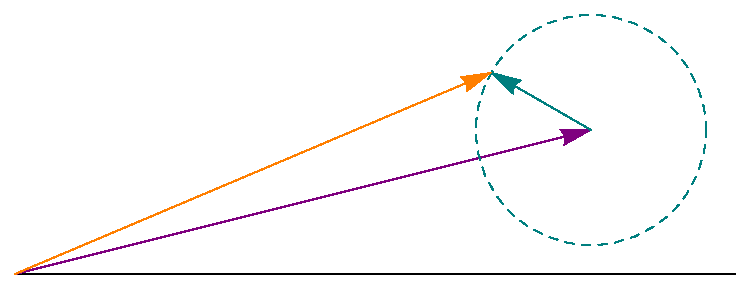
\includegraphics[scale=0.5]{body/image/FMnoise1.pdf}
        \hspace{30pt}
        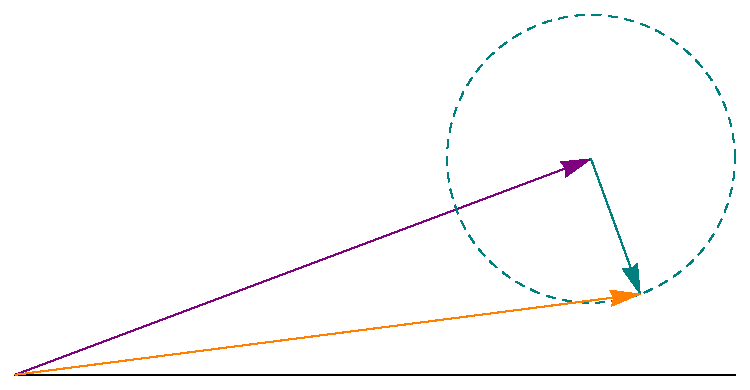
\includegraphics[scale=0.5]{body/image/FMnoise2.pdf}
        \caption{矢量合成示意图}
    \end{figure}

    得到$r(t)$类似于矢量和合成,如上图,在大信噪比下,不难知,新合成的的信号$B(t)$的相位为
    \begin{equation}
        \begin{split}
            \psi(t) &=\varphi(t)+\arctan\frac{V_n(t)\sin[\phi_n(t)-\varphi(t)]}{A_c+V_n(t)\cos[\phi_n(t)-\varphi(t)]}\\
                    &\approx\varphi(t)+\arctan\frac{V_n(t)\sin[\phi_n(t)-\varphi(t)]}{A_c}\\
                    &\approx\varphi(t)+\frac{V_n(t)\sin[\phi_n(t)-\varphi(t)]}{A_c}
        \end{split}
    \end{equation}
    因为AWGN是各向同性的,$\phi_n(t)$是在$[0,2\pi]$上的均匀分布,
    故$V_n(t)\sin[\phi_n(t)-\varphi(t)]$仍是$n_i(t)$的正交分量$n_s(t)$
    \footnote{当然也可以是同相分量$n_c(t)$,这里乘的是$\sin$,就姑且用正交分量了}。

    所以瞬时相位偏移
    \begin{equation}
        \psi(t)\approx\varphi(t)+\frac{n_s(t)}{A_c}
    \end{equation}

    鉴频器输出
    \begin{equation}
        y_o(t)=\frac{1}{2\pi}\frac{\dif}{\dif t}\psi(t)=\underbrace{K_fm(t)}_{\text{有用信号}}+\underbrace{\frac{1}{2\pi A_c}\frac{\dif n_s(t)}{\dif t}}_{\text{噪声}}
    \end{equation}

    输出信号的功率为$P_s=K_f^2P_m$,其带宽W,通过滤波器将噪声信号频域截短,其功率为
    \begin{equation}
        P_n=\left(\frac{1}{2\pi A}\right)^2\int_{-W}^{W}N_0\abs{j2\pi f}^2\dif f=\int_{-W}^{W}\frac{N_0f^2}{A^2}\dif f=\frac{2N_0W^3}{3A^2}
    \end{equation}

    可见解调输出信噪比为
    \begin{equation}
        \left(\frac{S}{N}\right)_o=\frac{3A^2K_f^2}{2W^2}\frac{P_m}{N_0W}=\frac{3A^2}{2}\left[\frac{\beta_f}{\text{max}\abs{m(t)}}\right]^2\frac{P_m}{N_0W}=3P_{m_n}\beta_f^2\frac{P_R}{N_0W}
    \end{equation}
    其中$P_{m_n}=\dfrac{P_m}{[\text{max}\abs{m(t)}]^2}$,是信号归一化之后的功率,也叫做调制信号功率的均峰比。
    特别的,对于单音正弦信号,$P_{m_n}=0.5$,则
    \begin{equation}
        \left(\frac{S}{N}\right)_o=1.5\beta_f^2\frac{P_R}{N_0W}
    \end{equation}
    
    FM的调制指数通常大于5,因此FM解调增益很大。FM信号带宽扩展倍数为$2\beta+2$,降低频谱效率换取抗干扰性能。

    相干解调无门限效应,包络检波存在门限效应。
    如果输入信号的信噪比不够大,比如小于一定的门限,则有用信号的相位会被"淹没"在噪声的相位里,造成接收机不能正常工作。

    
\subsection{各种模拟调制的对比}
    假设原信号$m(t)$为幅度为1、带宽为W的基带平稳过程,有$\mathscr{E}[m(t)]=0$,$\mathscr{E}[m^2(t)]=0.5$(如单音正弦信号)。
    接收机输入端有用信号的功率均为$P_R$。

    四种调制方式的解调输出信噪比为:
    \begin{align}
        &\left(\frac{S}{N}\right)_{\text{DSB}}=G_{\text{DSB}}\frac{P_R}{N_02W}=\frac{P_R}{N_0W}\\
        &\left(\frac{S}{N}\right)_{\text{SSB}}=\frac{P_R}{N_0W}\\
        &\left(\frac{S}{N}\right)_{\text{AM}}=\eta\left(\frac{S}{N}\right)_{\text{DSB}}=\frac{P_M}{1+P_M}\frac{P_R}{N_0W}=\frac{1}{3}\frac{P_R}{N_0W}\\
        &\left(\frac{S}{N}\right)_{\text{FM}}=3P_{m_n}\beta_f^2\frac{P_R}{N_0W}=1.5\beta_f^2\frac{P_R}{N_0W}
    \end{align}
    \begin{table}[H]
        \centering
        \caption{模拟调制的对比}
        \begin{tabular}{c|c|c|c}
            \Xhline{1pt}
            \textcolor{bupt}{调制}    & \textcolor{bupt}{传输带宽} & \textcolor{bupt}{设备复杂性}              & \textcolor{bupt}{主要应用}                    \\ \Xhline{0.5pt}
            \textcolor{bupt}{DSB}     &   2W                      & \parbox[t]{12em}{中等;要求相干解调}       & \parbox[t]{14em}{模拟数据传输,低带宽多路复用}  \\ \Xhline{0.5pt}
            \textcolor{bupt}{AM}      &   2W                      & \parbox[t]{12em}{较小;调制与解调简单}     & \parbox[t]{14em}{无线电广播系统}               \\ \Xhline{0.5pt}
            \textcolor{bupt}{SSB}     &   W                       & \parbox[t]{12em}{较大;调制解调都比较复杂} & \parbox[t]{14em}{音话通信、音话频分多路通信}     \\ \Xhline{0.5pt}
            \textcolor{bupt}{VSB}     &   略大于W                 & \parbox[t]{12em}{较大;需要对称滤波}       & \parbox[t]{14em}{数据传输、模拟电视}            \\ \Xhline{0.5pt}
            \textcolor{bupt}{FM}      &   2($\beta$+1)W           & \parbox[t]{12em}{中等;调制复杂,解调简单} & \parbox[t]{14em}{数据传输、无线广播、微波中继}   \\ \Xhline{1pt}
        \end{tabular}
    \end{table}